\section*{Abstract}
		This document presents the complete Lagrangian formulation of the T0 theory based on the fundamental geometric parameter $\xi = \frac{4}{3} \times 10^{-4}$. The theory establishes a fundamental time-mass duality $T(x,t) \cdot m(x,t) = 1$ and develops an extended Lagrangian with mass-proportional coupling to a dynamic time field. For the geometric derivation of the anomalous magnetic moments and experimental predictions, see Document 018\_T0\_Anomale-g2-10\_De.tex. The focus here lies on the field-theoretic structure and the derivation of the fundamental T0 contribution formula from first principles.

	
	
	\section{Introduction}
	
	\subsection{Basic Principles of the T0 Theory}
	
	The T0 theory postulates a fundamental duality between time and mass:
	\begin{equation}
		T(x,t) \cdot m(x,t) = 1
		\label{eq:time_mass_duality}
	\end{equation}
	
	This duality leads to several fundamental consequences:
	\begin{itemize}
		\item Natural mass hierarchy through time scales
		\item Dynamic mass generation through the time field
		\item Quadratic scaling of the anomalous magnetic moments with $m_\ell^2$
		\item Intrinsic integration of gravitation into quantum field theory
	\end{itemize}
	
	\subsection{The Fundamental Geometric Parameter}
	
	The entire T0 theory is based on a single fundamental parameter:
	\begin{equation}
		\boxed{\xi = \frac{4}{3} \times 10^{-4} = 1.333 \times 10^{-4}}
		\label{eq:xi_fundamental}
	\end{equation}
	
	This dimensionless parameter encodes the fundamental geometric structure of three-dimensional space. For the detailed geometric interpretation and derivation, see \href{https://github.com/jpascher/T0-Time-Mass-Duality/blob/main/2/pdf/018_T0_Anomale-g2-10_De.pdf}{Document 018}.
	
	\subsection{Notation and Conventions}
	
	We use natural units ($\hbar = c = 1$) with metric signature $(+,-,-,-)$:
	
	\begin{itemize}
		\item $T(x,t)$: Dynamic time field with $[T] = E^{-1}$
		\item $\delta E(x,t)$: Fundamental energy field with $[\delta E] = E$
		\item $\Delta m(x,t) = \delta E(x,t)$: Mass field fluctuations
		\item $\xi = 1.333 \times 10^{-4}$: Fundamental geometric parameter
		\item $\lambda$: base mass of the sector (appendix on $\lambda$; $m_P$ in the fundamental sector)
		\item $m_\ell$: Lepton masses ($e$, $\mu$, $\tau$)
	\end{itemize}
	
	\subsection{Derived Parameters}
	
	From the fundamental parameter $\xi$, the following are obtained:
	\begin{align}
		\xi^2 &= \left(1.333 \times 10^{-4}\right)^2 = 1.777 \times 10^{-8} \label{eq:xi_squared} \\
		\xi^4 &= \left(1.333 \times 10^{-4}\right)^4 = 3.160 \times 10^{-16} \label{eq:xi_fourth}
	\end{align}
	
	\section{Extended Lagrangian with Time Field}
	
	\subsection{Standard Model Lagrangian as Starting Point}
	
	The Standard Model Lagrangian for a lepton $\psi_\ell$ reads:
	\begin{equation}
		\mathcal{L}_{\text{SM}} = -\frac{1}{4} F_{\mu\nu}F^{\mu\nu} + \bar{\psi}_\ell(i\gamma^\mu D_\mu - m_\ell)\psi_\ell
		\label{eq:sm_lagrangian}
	\end{equation}
	
	where:
	\begin{itemize}
		\item $F_{\mu\nu} = \partial_\mu A_\nu - \partial_\nu A_\mu$: Electromagnetic field strength tensor
		\item $D_\mu = \partial_\mu + ie A_\mu$: Covariant derivative
		\item $m_\ell$: Lepton mass (constant)
	\end{itemize}
	
	\subsection{Introduction of the Dynamic Time Field}
	
	In the T0 theory, the mass is not constant but coupled to a dynamic time field $T(x,t)$ through the time-mass duality \eqref{eq:time_mass_duality}. We introduce the mass field:
	\begin{equation}
		m(x,t) = m_0 + \Delta m(x,t)
		\label{eq:mass_field}
	\end{equation}
	
	where $m_0$ is the rest mass and $\Delta m(x,t)$ represents the dynamic mass fluctuations.
	
	\subsection{Kinetic Term of the Time Field}
	
	The time field itself requires a kinetic term:
	\begin{equation}
		\mathcal{L}_{\text{kin}}^{(T)} = \frac{1}{2}(\partial_\mu \Delta m)(\partial^\mu \Delta m)
		\label{eq:time_field_kinetic}
	\end{equation}
	
	This term describes the propagation of mass field fluctuations as dynamic degrees of freedom.
	
	\subsection{Mass Term of the Time Field}
	
	The time field has a characteristic mass $m_T$:
	\begin{equation}
		\mathcal{L}_{\text{mass}}^{(T)} = -\frac{1}{2} m_T^2 \Delta m^2
		\label{eq:time_field_mass}
	\end{equation}
	
	The time field mass $m_T$ is given through the Higgs-time field connection by:
	\begin{equation}
		m_T = \frac{\lambda}{\xi}
		\label{eq:time_field_mass_value}
	\end{equation}
	
	where $\lambda$ is the base mass of the respective sector ($m_P$ in the fundamental sector); dimensionally $\lambda$ must be a mass, see the appendix on $\lambda$.
	
	\subsection{Mass-Proportional Coupling}
	
	The fundamental new term in the T0 theory is the coupling of the lepton fields to the time field, proportional to the lepton mass:
	\begin{equation}
		\mathcal{L}_{\text{int}} = g_T^\ell \, \bar{\psi}_\ell \psi_\ell \, \Delta m
		\label{eq:interaction_term}
	\end{equation}
	
	The coupling strength is given by:
	\begin{equation}
		\boxed{g_T^\ell = \xi \, m_\ell}
		\label{eq:coupling_strength}
	\end{equation}
	
	This mass-proportional coupling is the core of the T0 theory. It implies:
	\begin{itemize}
		\item Heavier leptons couple more strongly to the time field
		\item The coupling scales linearly with mass
		\item This leads to quadratic mass scaling in quantum corrections
	\end{itemize}
	
	\subsection{Complete Extended Lagrangian}
	
	The complete T0 Lagrangian combines all terms:
	\begin{equation}
		\begin{split}
			\mathcal{L}_{\text{T0}} = &-\frac{1}{4} F_{\mu\nu}F^{\mu\nu} \\
			&+ \bar{\psi}_\ell(i\gamma^\mu D_\mu - m_\ell)\psi_\ell \\
			&+ \frac{1}{2}(\partial_\mu \Delta m)(\partial^\mu \Delta m) \\
			&- \frac{1}{2} m_T^2 \Delta m^2 \\
			&+ \xi \, m_\ell \,\bar{\psi}_\ell \psi_\ell \, \Delta m
		\end{split}
		\label{eq:full_lagrangian}
	\end{equation}
	
	\section{Quantum Corrections and Feynman Rules}
	
	\subsection{Feynman Rules from the Lagrangian}
	
	From the interaction term \eqref{eq:interaction_term}, the Feynman rules follow:
	
	\textbf{Vertex factor:}
	\begin{equation}
		\bar{\psi}_\ell \psi_\ell \Delta m \quad \longrightarrow \quad -i g_T^\ell = -i \xi m_\ell
		\label{eq:vertex_factor}
	\end{equation}
	
	\textbf{Time field propagator:}
	\begin{equation}
		\Delta m(k) \quad \longrightarrow \quad \frac{i}{k^2 - m_T^2 + i\epsilon}
		\label{eq:propagator}
	\end{equation}
	
	\subsection{One-Loop Diagram}
	
	The fundamental one-loop diagram for the anomalous magnetic moment contribution has the structure:
\begin{center}
	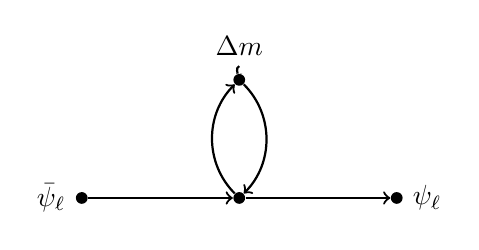
\begin{tikzpicture}[
		vertex/.style={circle,fill,inner sep=1.5pt},
		fermion/.style={->,thick},
		scalar/.style={dashed,thick}
		]
		% Vertices
		\node[vertex,label=left:$\bar{\psi}_\ell$] (a) at (0,0) {};
		\node[vertex] (b) at (2,0) {};
		\node[vertex,label=right:$\psi_\ell$] (c) at (4,0) {};
		\node[vertex] (d) at (2,1.5) {};
		
		% Lines
		\draw[fermion] (a) -- (b);
		\draw[fermion] (b) -- (c);
		\draw[fermion] (b) to[bend left=45] (d);
		\draw[fermion] (d) to[bend left=45] (b);
		\draw[scalar] (d) to[loop above,looseness=8] node[above] {$\Delta m$} (d);
	\end{tikzpicture}
\end{center}


	
	\subsection{General Formula for Scalar Mediators}
	
	For a scalar mediator with mass $m_T$ and coupling $g_T^\ell$, the general one-loop formula reads:
	\begin{equation}
		\begin{split}
			\Delta a_\ell = \frac{(g_T^\ell)^2}{8\pi^2} \int_0^1 dx \, 
			\frac{m_\ell^2 (1-x)(1-x^2)}{m_\ell^2 x^2 + m_T^2 (1-x)}
		\end{split}
		\label{eq:general_loop_formula}
	\end{equation}
	
	\textbf{Restriction:} numerator and denominator of this formula come from two different parametrizations. The standard form for a scalar mediator is $\Delta a_\ell = \frac{(g_T^\ell)^2}{8\pi^2}\int_0^1 dx\,\frac{m_\ell^2(1-x)^2(1+x)}{m_\ell^2(1-x)^2 + m_T^2\,x}$; in the limit $m_T \gg m_\ell$ it gives $\frac{(g_T^\ell)^2 m_\ell^2}{8\pi^2 m_T^2}\bigl(\ln\frac{m_T^2}{m_\ell^2} - \frac76\bigr)$, not $\cdot\frac23$ (numerically for $m_T/m_\ell = 1000$: $12.65$ instead of $0.667$). The factor $2/3$ in the following section, and hence the prefactor of the T0 formula, rest on the mixed integrand; the $m_\ell^2$ scaling remains up to the logarithm.
	
	\section{Derivation of the Fundamental T0 Formula}
	
	\subsection{Heavy Mediator Limit}
	
	For $m_T \gg m_\ell$, the integral \eqref{eq:general_loop_formula} can be simplified. In the denominator, the term $m_T^2 (1-x)$ dominates:
	\begin{equation}
		\frac{m_\ell^2 (1-x)(1-x^2)}{m_\ell^2 x^2 + m_T^2 (1-x)} 
		\approx \frac{m_\ell^2 (1-x)(1-x^2)}{m_T^2 (1-x)} 
		= \frac{m_\ell^2 (1-x^2)}{m_T^2}
		\label{eq:heavy_mediator_approx}
	\end{equation}
	
	This yields:
	\begin{equation}
		\begin{split}
			\Delta a_\ell &\approx \frac{(g_T^\ell)^2 m_\ell^2}{8\pi^2 m_T^2} \int_0^1 dx \, (1-x^2) \\
			&= \frac{(g_T^\ell)^2 m_\ell^2}{8\pi^2 m_T^2} \left[x - \frac{x^3}{3}\right]_0^1 \\
			&= \frac{(g_T^\ell)^2 m_\ell^2}{8\pi^2 m_T^2} \left(1 - \frac{1}{3}\right) \\
			&= \frac{(g_T^\ell)^2 m_\ell^2}{8\pi^2 m_T^2} \cdot \frac{2}{3}
		\end{split}
		\label{eq:integral_evaluation}
	\end{equation}
	
	\subsection{Inserting the T0 Coupling}
	
	With the coupling acting in the interaction term as the dimensionless $\xi$, we obtain:
	\begin{equation}
		\begin{split}
			\Delta a_\ell &= \frac{\xi^2 m_\ell^2}{8\pi^2 m_T^2} \cdot \frac{2}{3} \\
			&= \frac{2 \xi^2 m_\ell^2}{24\pi^2 m_T^2} \\
			&= \frac{\xi^2 m_\ell^2}{12\pi^2 m_T^2}
		\end{split}
		\label{eq:t0_coupling_inserted}
	\end{equation}
	With $m_\ell^2$ from the loop integral, the result is dimensionless and quadratic in $m_\ell$ only if the coupling in the interaction term acts as the dimensionless $\xi$; $g_T^\ell = \xi m_\ell$ would have the dimension of a mass and would give $m_\ell^4$ with $[\Delta a] = E^2$. The mass proportionality thus resides in the loop factor $m_\ell^2$.
	
	\subsection{Higgs-Time Field Connection}
	
	With the time field mass \eqref{eq:time_field_mass_value}, this becomes:
	\begin{equation}
		\begin{split}
			\Delta a_\ell &= \frac{\xi^2 m_\ell^2}{12\pi^2 (\lambda/\xi)^2} \\
			&= \frac{\xi^2 m_\ell^2}{12\pi^2} \cdot \frac{\xi^2}{\lambda^2} \\
			&= \frac{\xi^4 m_\ell^2}{12\pi^2 \lambda^2}
		\end{split}
		\label{eq:higgs_connection_substituted}
	\end{equation}
	
	\subsection{Final Formula}

	Eq.~\eqref{eq:higgs_connection_substituted} is already the final formula of the limit $m_T \gg m_\ell$:
	\begin{equation}
		\boxed{\Delta a_\ell^{\text{(T0)}} = \frac{\xi^4}{12\pi^2\lambda^2} \cdot m_\ell^2}
		\label{eq:t0_fundamental_formula}
	\end{equation}
	The prefactor $1/12$ rests on the factor $2/3$ from the mixed integrand (see the section \enquote{General Formula for Scalar Mediators}); with the standard form, $\ln(m_T^2/m_\ell^2) - 7/6$ takes its place.

	$\Delta a_\ell$ is dimensionless exactly when $\lambda$ is a mass -- this is the reading of the appendix on $\lambda$: $\lambda = M_\text{base}$, in the fundamental sector $M_\text{base} = m_P$.

	\section{Numerical Evaluation}

	\subsection{Determination of the Normalization Constant}

	The normalization constant reads:
	\begin{equation}
		C_{\text{T0}} = \frac{\xi^4}{12\pi^2\lambda^2}
		\label{eq:normalization_constant}
	\end{equation}

	With $\xi^4 = 3.160 \times 10^{-16}$ and $\lambda = m_P = 1.221 \times 10^{19}$~GeV (appendix on $\lambda$) we obtain:
	\begin{equation}
		C_{\text{T0}} = \frac{3.160 \times 10^{-16}}{118.4 \times 1.491 \times 10^{38}\ \text{GeV}^2} = 1.79 \times 10^{-56} \text{ GeV}^{-2}
		\label{eq:numerical_constant}
	\end{equation}

	\subsection{Final T0 Contribution Formula}

	The fully evaluated T0 contribution formula reads:
	\begin{equation}
		\boxed{\Delta a_\ell^{\text{(T0)}} = 1.79 \times 10^{-56} \cdot m_\ell^2 \text{ [GeV}^{-2}\text{]}}
		\label{eq:final_t0_formula}
	\end{equation}

	where $m_\ell$ is to be inserted in GeV.

	\subsection{Lepton-Specific Predictions}

	With the lepton masses:
	\begin{itemize}
		\item $m_e = 0.511$ MeV $= 0.000511$ GeV
		\item $m_\mu = 105.658$ MeV $= 0.105658$ GeV
		\item $m_\tau = 1776.86$ MeV $= 1.77686$ GeV
	\end{itemize}

	the T0 contributions are:

	\textbf{Electron:}
	\begin{equation}
		\begin{split}
			\Delta a_e^{\text{(T0)}} &= 1.79 \times 10^{-56} \cdot (0.000511)^2 \\
			&= 1.79 \times 10^{-56} \cdot 2.611 \times 10^{-7} \\
			&= 4.7 \times 10^{-63}
		\end{split}
		\label{eq:electron_prediction}
	\end{equation}

	\textbf{Muon:}
	\begin{equation}
		\begin{split}
			\Delta a_\mu^{\text{(T0)}} &= 1.79 \times 10^{-56} \cdot (0.105658)^2 \\
			&= 1.79 \times 10^{-56} \cdot 1.1164 \times 10^{-2} \\
			&= 2.0 \times 10^{-58}
		\end{split}
		\label{eq:muon_prediction}
	\end{equation}

	\textbf{Tau:}
	\begin{equation}
		\begin{split}
			\Delta a_\tau^{\text{(T0)}} &= 1.79 \times 10^{-56} \cdot (1.77686)^2 \\
			&= 1.79 \times 10^{-56} \cdot 3.1572 \\
			&= 5.7 \times 10^{-56}
		\end{split}
		\label{eq:tau_prediction}
	\end{equation}

	\subsection{No Conversion Needed}

	The anomalous magnetic moment $a_\ell = (g_\ell - 2)/2$ is dimensionless; the values above are already the values to be compared with experiment (often quoted in units of $10^{-11}$). The Lagrangian contribution of the time field is thus many orders of magnitude below any measurement precision.

	With the Fermilab final result and the 2025 White Paper of the Muon~$g-2$ Theory Initiative, the deviation between the measured $a_\mu$ and the Standard Model prediction is no longer significant; the current status is given in Doc.~382. A negligible Lagrangian contribution does not contradict this.

	\section{Quadratic Mass Scaling}
	
	\subsection{Fundamental Prediction}
	
	The central prediction of the T0 theory is the quadratic mass scaling \eqref{eq:final_t0_formula}:
	\begin{equation}
		\Delta a_\ell^{\text{(T0)}} \propto m_\ell^2
		\label{eq:quadratic_scaling}
	\end{equation}
	(with the standard form of the loop integral, up to the factor $\ln(m_T^2/m_\ell^2)$, see the section \enquote{General Formula for Scalar Mediators}).
	
	This leads to natural hierarchies:
	\begin{align}
		\frac{\Delta a_e^{\text{(T0)}}}{\Delta a_\mu^{\text{(T0)}}} 
		&= \left(\frac{m_e}{m_\mu}\right)^2 
		= \left(\frac{0.511}{105.658}\right)^2 
		= 2.34 \times 10^{-5} \label{eq:electron_muon_ratio} \\
		\frac{\Delta a_\tau^{\text{(T0)}}}{\Delta a_\mu^{\text{(T0)}}} 
		&= \left(\frac{m_\tau}{m_\mu}\right)^2 
		= \left(\frac{1776.86}{105.658}\right)^2 
		= 282.8 \label{eq:tau_muon_ratio}
	\end{align}
	
	\subsection{Physical Interpretation}
	
	The quadratic mass scaling has deep physical significance:
	
	\textbf{Cause:} The mass proportionality resides in the factor $m_\ell^2$ of the loop integral, while the coupling in the interaction term acts as the dimensionless $\xi$; thus $\xi^2 m_\ell^2$ appears in the one-loop contribution.
	
	\textbf{Consequences:}
	\begin{itemize}
		\item Electron effects are smaller by $\sim 10^{-5}$ relative to the muon
		\item Muon effects are of order $\sim 10^{-58}$ and not measurable
		\item Tau effects are relatively the largest ($\sim 280 \times$ larger than muon), in absolute terms also negligible
	\end{itemize}
	
	\textbf{Comparison with QED:} In the Standard Theory, the leading contribution scales as $\alpha/(2\pi)$, independent of the mass. The T0 theory adds a mass-dependent contribution.
	
	\section{Connection to the Geometric Formulation}
	
	\subsection{Relation to the g-2 Analysis}
	
	The T0 contributions $\Delta a_\ell^{\text{(T0)}}$ derived here are additional contributions to the Standard Model. They are \textbf{not} the same quantities as the values geometrically derived in Document 018: Doc.~018 obtains $\Delta a(\mu{-}e) = 4.37 \times 10^{-6}$ from $4\pi/f^{p}$, whereas here a contribution $\propto m_\ell^2$ of $\sim 10^{-58}$ results. The two formulations give contributions differing by many orders of magnitude, with different mass dependence. The load-bearing g-2 line is the ratio line in Docs.~018 and 158.

	\textbf{On notation:} here $f$ is the base winding number $f = 1/\xi = 7500$, not a frequency. In natural units $f$ is only another reading of the duality $T\cdot m = 1$: $f = t_P/t_0 = \Lambda_{\text{T0}}/E_P$ with $t_0 = \xi\,t_P$ and $\Lambda_{\text{T0}} = E_P/\xi$, and $\xi E_0^2 = 1$ gives $f = E_0^2$. As a dimensionless ratio, $f$ cannot be set to~1 with justification (Doc.~A135).

	The difference in notation:
	\begin{itemize}
		\item \textbf{Document 018:} Calculates directly $a_\ell$ (including SM + T0)
		\item \textbf{This document:} Calculates $\Delta a_\ell^{\text{(T0)}}$ (T0 contribution only)
	\end{itemize}
	
	The relation is:
	\begin{equation}
		a_\ell^{\text{(total)}} = a_\ell^{\text{(SM)}} + \Delta a_\ell^{\text{(T0)}}
		\label{eq:total_relation}
	\end{equation}
	
	\subsection{Parameter Correspondences}
	
	The geometric parameters from Document 018 correspond to the Lagrangian parameters:
	\begin{align}
		\xi &= \frac{4}{3} \times 10^{-4} \quad \text{(identical in both formulations)} \label{eq:xi_correspondence} \\
		f &= 7500 \quad \text{(geometric sub-Planck factor)} \label{eq:f_correspondence} \\
		\varphi &= \frac{1+\sqrt{5}}{2} \quad \text{(pentagonal symmetry breaking)} \label{eq:phi_correspondence}
	\end{align}
	
	What the two formulations share is the parameter $\xi$; there is no numerical connection between the contributions (see above). The projection factor $k_{\text{geom}}$ belongs solely to the geometric 4D-3D projection in Doc.~018.
	
	\section{Higgs Mechanism in the T0 Theory}
	
	\subsection{Higgs Field as Fundamental Basis}
	
	In the T0 theory, the Higgs field is not an additional field but the fundamental basis of the time-mass duality:
	\begin{equation}
		T(x,t) \cdot m(x,t) = 1
		\label{eq:higgs_foundation}
	\end{equation}
	
	The universal parameter $\xi$ follows directly from the Higgs parameters:
	\begin{equation}
		\boxed{\xi = \frac{\lambda_h^2 v^2}{16\pi^3 m_h^2}}
		\label{eq:xi_from_higgs}
	\end{equation}
	
	with:
	\begin{itemize}
		\item $\lambda_h$: Higgs self-coupling
		\item $v = 246$ GeV: Higgs vacuum expectation value
		\item $m_h = 125$ GeV: Higgs mass
	\end{itemize}
	
	\subsection{Spontaneous Symmetry Breaking}
	
	The spontaneous symmetry breaking of the Higgs field generates:
	\begin{itemize}
		\item Lepton masses through Yukawa coupling
		\item The time field $T(x,t)$ as fluctuations around the VEV
		\item The time-mass duality as fundamental structure
	\end{itemize}
	
	In this picture, mass fluctuations $\Delta m$ are directly connected to Higgs fluctuations:
	\begin{equation}
		\Delta m(x,t) = y_\ell \cdot \delta h(x,t)
		\label{eq:higgs_fluctuation}
	\end{equation}
	
	where $y_\ell$ is the Yukawa coupling and $\delta h$ is the Higgs fluctuation.
	
	\section{Field-Theoretic Structure}
	
	\subsection{Equations of Motion}
	
	From the Lagrangian \eqref{eq:full_lagrangian}, the Euler-Lagrange equations follow:
	
	\textbf{For the lepton field:}
	\begin{equation}
		(i\gamma^\mu D_\mu - m_\ell + \xi m_\ell \Delta m)\psi_\ell = 0
		\label{eq:lepton_eom}
	\end{equation}
	
	\textbf{For the time field:}
	\begin{equation}
		\Box \Delta m + m_T^2 \Delta m = \xi m_\ell \bar{\psi}_\ell \psi_\ell
		\label{eq:time_field_eom}
	\end{equation}
	
	where $\Box = \partial_\mu \partial^\mu$ is the d'Alembert operator.
	
	\subsection{Interpretation of the Equations of Motion}
	
	Equation \eqref{eq:lepton_eom} shows that the lepton has an effective mass:
	\begin{equation}
		m_{\text{eff}}(x,t) = m_\ell (1 - \xi \Delta m)
		\label{eq:effective_mass}
	\end{equation}
	The sign follows from $\mathcal{L}_{\text{int}} = +\xi m_\ell\bar\psi_\ell\psi_\ell\Delta m$: $\partial\mathcal{L}/\partial\bar\psi_\ell = (i\gamma^\mu D_\mu - m_\ell + \xi m_\ell\Delta m)\psi_\ell$.
	
	The mass is modulated by the time field.
	
	Equation \eqref{eq:time_field_eom} shows that the time field has a source:
	\begin{equation}
		\text{Source} = \xi m_\ell \bar{\psi}_\ell \psi_\ell = \xi m_\ell \rho_\ell
		\label{eq:source_term}
	\end{equation}
	
	The lepton density $\rho_\ell$ generates time field fluctuations, proportional to the lepton mass.
	
	\subsection{Energy Scales}
	
	The characteristic energy scales in the theory are:
	\begin{align}
		E_{\text{Lepton}} &\sim m_\ell \quad \text{(lepton mass)} \label{eq:lepton_scale} \\
		E_{\text{Time}} &\sim m_T = \frac{\lambda}{\xi} \quad \text{(time field mass)} \label{eq:time_scale} \\
		E_{\text{Coupling}} &\sim \xi m_\ell \ll m_\ell \quad \text{(weak coupling)} \label{eq:coupling_scale}
	\end{align}
	
	The hierarchy $E_{\text{Coupling}} \ll E_{\text{Lepton}} \ll E_{\text{Time}}$ justifies the perturbative treatment.
	
	\section{Renormalization (historical presentation)}

\textbf{Note:} This section uses the language of QFT renormalization (wavefunction renormalization, $\beta$-function, RG equations) as a descriptive tool. In the complete FFGFT formulation (Doc.~202), traditional renormalization is not required: the fractal torus provides a natural UV cutoff at $E_P/\xi$, and the scale structure follows from the recursion $\mathcal{R}$. The formulae used here are compatible with the FFGFT structure, but the terminology is closer to SM language than to native FFGFT language.
	
	\subsection{Divergences in Loop Diagrams}
	
	The one-loop integral \eqref{eq:general_loop_formula} is finite for $m_T \gg m_\ell$. However, higher orders may contain divergences.
	
	The renormalization of the T0 theory requires:
	\begin{itemize}
		\item Wave function renormalization for $\psi_\ell$ and $\Delta m$
		\item Mass renormalization for $m_\ell$ and $m_T$
		\item Coupling renormalization for $g_T^\ell$
	\end{itemize}
	
	\subsection{Renormalization Group Equations}
	
	The running coupling follows:
	\begin{equation}
		\mu \frac{d g_T^\ell}{d\mu} = \beta_{g_T}(g_T^\ell)
		\label{eq:rg_equation}
	\end{equation}
	
	Due to the mass-proportional structure \eqref{eq:coupling_strength}:
	\begin{equation}
		\beta_{g_T} = \xi \beta_m
		\label{eq:beta_relation}
	\end{equation}
	
	where $\beta_m$ is the anomalous mass dimension.
	
	\subsection{Consistency with the Standard Model}
	
	The T0 contributions are subdominant compared to the Standard Model contributions:
	\begin{equation}
		\frac{\Delta a_\ell^{\text{(T0)}}}{a_\ell^{\text{(QED)}}} \sim \frac{\xi^4 m_\ell^2}{6\pi\alpha\lambda^2} \ll 1
		\label{eq:hierarchy}
	\end{equation}
	
	The expression follows with $a^\text{(QED)} \approx \alpha/(2\pi)$ and Eq.~\eqref{eq:t0_fundamental_formula}; only with $\lambda^2$ is it dimensionless.

	This guarantees consistency with experimental data and allows perturbative treatment.
	
	\section{Comparison of Different Formulations}
	
	\subsection{Lagrangian vs. Geometric Formulation}
	
	\begin{table}[h]
		\centering
		\adjustbox{max width=\textwidth}{%
\begin{tabular}{lcc}
			\toprule
			\textbf{Aspect} & \textbf{Lagrangian (Doc. 019)} & \textbf{Geometric (Doc. 018)} \\
			\midrule
			Starting point & Time field $\Delta m(x,t)$ & Torsion lattice, windings \\
			Method & Field theory, loop integrals & Fractal geometry \\
			Main formula & $\Delta a \propto \xi^4 m^2$ & $a_e = S_3/(f\,k_\text{eff})$, $\Delta a = 4\pi/f^{p}$ \\
			Prediction & T0 contribution $\Delta a$ & Total value $a$ \\
			Parameters & $\xi$, $\lambda$, $m_T$ & $\xi$, $\varphi$, $f$ \\
			\bottomrule
		\end{tabular}%
}
		\caption{Comparison of formulations}
		\label{tab:comparison}
	\end{table}
	
	\subsection{Complementarity}
	
	The two formulations are complementary:
	\begin{itemize}
		\item \textbf{Lagrangian:} Provides the field-theoretic structure and Feynman rules
		\item \textbf{Geometric:} Provides the physical intuition and ratio predictions
	\end{itemize}
	
	The numerical predictions for $a_\ell$ come from the geometric formulation (Docs.~018, 158); the Lagrangian contribution of the time field is negligibly small (see the section \enquote{Relation to the g-2 Analysis}).
	
	\section*{Bibliography}
	
	\begin{thebibliography}{99}
		
		\bibitem{t0_g2_2026}
		J. Pascher,
		\textit{Anomalous Magnetic Moments in the FFGFT Theory: Geometric Derivation from the Time-Mass Duality},
		\href{https://github.com/jpascher/T0-Time-Mass-Duality/blob/main/2/pdf/018_T0_Anomale-g2-10_De.pdf}{Document 018\_T0\_Anomale-g2-10\_De.pdf},
		February 2026.
		
		\bibitem{peskin_schroeder_1995}
		M. E. Peskin, D. V. Schroeder,
		\textit{An Introduction to Quantum Field Theory},
		Westview Press, 1995.
		Standard reference for Feynman rules and loop calculations.
		
		\bibitem{pdg_2024}
		Particle Data Group,
		\textit{Review of Particle Physics},
		Prog. Theor. Exp. Phys. 2024, 083C01 (2024).
		Experimental values for lepton masses and g-2.
		
		\bibitem{higgs_1964}
		P. W. Higgs,
		\textit{Broken Symmetries and the Masses of Gauge Bosons},
		Phys. Rev. Lett. 13, 508 (1964).
		Original Higgs mechanism.
		
		\bibitem{weinberg_qft}
		S. Weinberg,
		\textit{The Quantum Theory of Fields, Volume I: Foundations},
		Cambridge University Press, 1995.
		Comprehensive treatment of quantum field theory.
		
	\end{thebibliography}

\section*{Appendix on $\lambda$: Meaning of $\lambda$ in $m_T = \lambda/\xi$}

In the formula $m_T = \lambda/\xi$, $\lambda$ is not the Higgs coupling parameter.

\textbf{Three reasons:}
(i)~Dimensionally, $\lambda$ must be a \emph{mass}, since $m_T$ is a mass
and $\xi$ is dimensionless; the Higgs quartic $\lambda_h \approx 0.129$
is dimensionless.
(ii)~$\lambda_h$ runs under the RGE and is a low-energy parameter of the
electroweak scale; a value measured there cannot be inserted at the Planck scale.
(iii)~Interpreted as a dimensionless factor in Planck units, $\lambda_h$
would give range $7.75\cdot L_0$ --- misses $L_0$.

\textbf{Correct:} $\lambda = M_\text{basis}$ is the basis mass of the respective
sector; in the fundamental sector $M_\text{basis} = m_P$ (R89/R90, Doc.~180).
The formula reads structurally $m_T = M_\text{basis}/\xi$, sector-dependent
value, universal form.
